\documentclass[conference]{IEEEtran}
\IEEEoverridecommandlockouts
\usepackage{cite,amsmath,amssymb,graphicx,booktabs,xcolor,balance}
\usepackage[caption=false,font=footnotesize]{subfig}
\usepackage{siunitx}
\sisetup{detect-all,group-separator={,}}
\usepackage{tikz}
\usetikzlibrary{arrows.meta,positioning,fit,backgrounds,calc}
\usepackage[hidelinks]{hyperref}

% Inherit the surrounding size: hardcoding \footnotesize made rule names
% 8 pt Helvetica inside a 7 pt table and oversized in figure annotations.
\newcommand{\rulename}[1]{\textsf{#1}}
% Every headline number is written \artv{key}{rendered}, which typesets only the second
% argument. paper/scripts/check_banlist.py parses these sites and asserts each rendered value
% equals the corresponding field of evaluation/results/final_summary.json. The previous gate
% asserted only that the artifact's value appeared SOMEWHERE in the sources, which a reviewer
% defeated twice over: "17" was satisfied by the seventeen fault classes, and a moved
% false-halt rate of 0.038 was satisfied by Fig. 2's ICC coordinate (0.038,0.05). Presence
% anywhere is not agreement here; this binds the number to the claim that makes it.
\newcommand{\artv}[2]{#2}

\begin{document}

\title{Orbit-Evidence: Relational Validity Checks for\\
Learning-Assisted Satellite Communication Experiments}

\author{\IEEEauthorblockN{Anonymous Submission}}

\maketitle

\begin{abstract}
Chronological train/validation/test splitting does not establish every property a deployment
claim needs, and some of those properties cannot be established from a single run at all: they
are relations \emph{between} executions. We formulate two such properties and make both
executable. \emph{Provenance completeness}: if two runs differ in output under an identical
declared provenance closure, the closure is incomplete---refutable differentially, never by
inspecting a manifest. \emph{Statistical-unit adequacy}: the chosen unit must be checked for
residual dependence at the next coarser physical level, which we decide against a permutation
reference with three outcomes rather than two---\textsc{pass}, \textsc{halt}, and
\textsc{indeterminate} when the design cannot support a decision at all. Satellite software supplies the obligations these sit among: an element set carries an epoch and a separate catalogue publication time, schedules exist only inside predicted-visible geometry, labels arrive when a catalogue publishes, and passes from one element set are repeated measures. Orbit-Evidence packages this as nineteen rules in four layers behind a CI gate. The unit rule is the one component whose error rates we measure: \num{14} false halts over \num{450} clean replicates, $0.031$, consistent with a nominal $0.05$ rather than better than it, with power $1.00$ at intraclass correlation $0.8$ but $0.25$ at $0.2$, falling to the false-halt rate below about $0.1$; the sweep runs in under \qty{2}{\second}. A curated seventeen-fault suite gives regression coverage of the represented violations---not completeness, not sensitivity, and no radio-frequency or learned-method claim.
\end{abstract}

\begin{IEEEkeywords}
experiment validity, data leakage, reproducibility, non-terrestrial networks,
learning-assisted communication, regression testing
\end{IEEEkeywords}

\section{Introduction}

Learning components are increasingly proposed as assistants to physical models in satellite
and non-terrestrial communication software: correcting a propagated orbital prediction,
adapting a link parameter, or deciding whether a learned branch should override a model-based
default~\cite{lin2021ntn}. Because such systems are temporal, evaluation is
organised as a chronological split---train on the past, validate on the near future, test on
the far future. That is a common and necessary practice for temporal learning pipelines, and
the conditions under which ordered splitting is valid are well
established~\cite{bergmeir2012crossval}.

Our claim is that it is not sufficient, and that the gap is one of kind rather than degree. A
chronological split constrains the \emph{order} of quantities already in a dataset, and is silent
on four further questions. \emph{Availability}: a quantity may be past-dated and still
unpublished, so no system could have held it. \emph{Membership}: which rows exist can itself be
decided by later data, in both directions, and a split cannot examine rows never created.
\emph{Hidden state}: a split governs rows, whereas information travels through a feature tensor,
a scaler, a coefficient vector, a tracker's latent state, selection metadata, or an admission
bit---none of which is a column. \emph{Statistical units}: a split says nothing about whether the unit over
which uncertainty is computed is exchangeable.

\subsection{Why the satellite domain makes this concrete}
\label{sec:whysat}

These gaps are abstract in general and specific here. Six properties of satellite communication
software give each protected object an operational meaning, and are why we develop the contract in
this domain rather than as generic tooling.

\emph{(i) Two clocks.} An orbital element set has an \emph{element epoch}---the instant its state vector describes---and a separate \emph{publication time}, carried as \texttt{CREATION\_DATE} and exposed per element set by the public catalogue~\cite{ccsds502omm,spacetrackgp}; they typically differ by hours, with a tail to days. A feature formed from two element epochs is a difference of two past timestamps: it passes every ordering test and is still unavailable if either was published after the decision instant. \emph{(ii) A decision instant that is a real endpoint.} Open-loop decisions use the state an
endpoint \emph{holds}, not the best that exists; staleness is normal, so availability is
first-class.
\emph{(iii) Schedules live inside predicted geometry}---a supporting physical obligation rather than one of the six objects. An opportunity exists only where the link is predicted visible above an elevation mask, so sampling a uniform grid and filtering afterwards yields rows no scheduler would emit. \emph{(iv) Labels arrive retrospectively, from a publisher.} A better-determined later element
set can serve as a label, but whether and when it appears is the catalogue's decision; later data
may set a label's value, uncertainty or closure time, and must never decide whether a row existed. \emph{(v) Repeated measures nest.} Samples in one pass share geometry and one propagation state, and every pass propagated from one element set shares that set's largely along-track error, so the exchangeable unit is usually the \emph{element set}, not the pass. Naming the level is the difficulty, which is why \rulename{L4.7} tests it rather than assuming it.
\emph{(vi) State survives a nominal freeze.} Stateful link adaptation and residual trackers update
at their own refresh events, which can fall after a model is declared frozen---so the learner keeps
observing outcomes even when the feature tensor is clean.

We therefore treat experimental validity as an \emph{executable contract}: each rule protects a
named object, states a violation, and is enforced by a check naming the rule it broke. Our thesis: Orbit-Evidence turns deployment-time
availability, row membership, model-state and statistical-unit assumptions into executable CI
checks for satellite communication experiments, and a curated regression suite demonstrates
those checks on seventeen known fault classes that chronological ordering alone is not
designed to detect.

\textbf{Contributions.}
\begin{enumerate}
\item \textbf{Validity conditions that are not predicates on one table.} Most checks test values
inside a dataset. Five of ours cannot be written that way. Four compare \emph{executions}:
recompute a feature with state after $t$ truncated and require bit-identity (\rulename{L1.1});
rebuild a registry from a truncated source under the same declared window (\rulename{L1.4});
require a probe mutation to change an observable before its non-detection means anything
(\rulename{L3.2}); and refute a provenance closure when two runs differ in output under an
identical manifest hash, the converse being merely redundant (\rulename{L4.6})---an asymmetry
that makes the property falsifiable without enumerating the input space. The fifth compares
\emph{aggregation levels}: \rulename{L4.7} tests whether the chosen unit stays exchangeable one
level coarser, with an explicit \textsc{indeterminate} outcome. Neither its estimator nor its
permutation test is new; treating the calibrated test, its operating characteristic and its
abstention state as a workflow gate is.
\item \textbf{A satellite experiment contract, and Orbit-Evidence.} Nineteen executable rules over
six protected objects in four layers (Table~\ref{tab:rules}), separating \emph{core} obligations
from \emph{support} rules that make the experiment auditable rather than following from deployment
causality. The domain supplies the obligations: element epoch versus catalogue publication,
predicted-visible scheduling, freeze-then-label membership, state crossing a nominal freeze, and
the element set as statistical unit. A \artv{source_loc}{\num{833}}-line \texttt{numpy}-only package.
\item \textbf{Calibrated executable evidence.} For \rulename{L4.7}, a measured false-halt rate and
a measured power curve with a deterministic abstention boundary (Fig.~\ref{fig:opcurve})---the only
component whose error rates are measured rather than assumed. Around it, curated regression coverage of seventeen fault
classes in three deterministic environments (Table~\ref{tab:rules}): the represented violations
cannot silently return, which is not sensitivity to faults the suite lacks (\S\ref{sec:threats}).
\end{enumerate}

We claim nothing about radio-frequency or packet-level performance. No learned communication
method is shown here to work or to fail; the object of study is the experiment, not the model.

\emph{Availability.} The toolkit, fixtures, fault suite and summary artifact accompany this
submission anonymously. \texttt{make gate} regenerates the evaluation, \rulename{L4.7}'s
operating characteristic included, and refuses to build if any headline number \emph{disagrees}
with the artifact at the sentence claiming it, if such a sentence is missing, if a retracted claim
reappears, or if a stated bound is exceeded---agreement per claim, not presence somewhere in the
sources. It is still a regression guard, not a proof of correctness: a wrong number that no rule
names would pass it.

\section{Threat Model and Experiment Contract}

\subsection{Decision time and the six protected objects}

Let $t_d$ be the \emph{decision instant}: the moment a deployed system must act using only
state it already holds---for an open-loop satellite endpoint, when a transmission is
committed from the element set on board. A deployment claim is interpretable only if every
quantity entering the decision was obtainable before $t_d$. Six objects are therefore
\emph{protected}; Fig.~\ref{fig:contract} shows their relationship in time.

Each object is the obligation one domain property of
\S\ref{sec:whysat} imposes; the parenthetical names which. \emph{Feature availability} and the
\emph{availability clock} (i): a feature must be computable from state available at $t_d$, selected
on publication rather than the descriptive clock. The adversarial case is not a future-dated
feature---ordering catches that---but one built from two past timestamps, one published after
$t_d$. \emph{Row membership} (iv): later information may change a label's status, value,
uncertainty or closure time, never whether a row exists; violations run both ways, rows dropped
when a later reference fails to appear and rows created when a schedule's extent comes from the
data on hand. \emph{Label closure} (iv): a retrospective label is usable only from $t_c$, and use
before it is the one ordering violation a split does catch---dotted in Fig.~\ref{fig:contract}.
The harder failure is when the \emph{probability} that a label exists depends on the covariate
under study, which no split addresses. \emph{State channels} (vi): information also enters through
the feature tensor, scaler, coefficients, a tracker's latent state, selected-model
metadata~\cite{cawley2010selection} or the gate bit---the six probed channels, an operational
enumeration, not a completeness claim. \emph{Statistical units} (v): replicates of one physical
event are not independent observations, and aggregating somewhere does not establish that level is
exchangeable. Predicted-visible geometry (iii) is a supporting physical obligation, not a seventh
object.

\subsection{Four layers}

The six objects do not partition the nineteen rules, and we do not claim they do. Six protect one
directly---\rulename{L1.1}--\rulename{L1.4}, \rulename{L3.1}, \rulename{L4.7}---and the rest are
the layers those obligations need to be checkable at all. L2 is domain sanity: a schedule must lie inside
geometry that can carry the link (\S\ref{sec:whysat}\,iii), the target between a resolution floor
and a plausibility ceiling, declared relations must match implementations. L3 adds the
canary-effectiveness precondition, without which an inert probe reads as an absent leak, and L4 is
reproducibility hygiene, independent of the causal model rather than derived from it.

Two design commitments make the contract usable. Every violation raises an exception carrying its
\emph{rule identifier}, so a finding names what it broke instead of surfacing a bare assertion
failure. And a detector is trusted only once demonstrated to fail on a deliberately broken
fixture---a check that cannot go red is not evidence---which Table~\ref{tab:rules} reports per
layer.

\subsection{Relation to existing practice}

Most of what follows is not new in isolation, and we state the delta rather than the territory.
Executable production-readiness
rubrics~\cite{breck2017mltestscore,polyzotis2019datavalidation}, point-in-time correctness in
feature stores, hidden-state leakage as configuration coupling~\cite{sculley2015debt},
pseudoreplication~\cite{hurlbert1984pseudoreplication}, boundary-value analysis, and leakage
taxonomies~\cite{kaufman2012leakage} with surveys of prevalence~\cite{kapoor2023leakage} all
predate us; time-series work establishes when ordered splitting is
valid~\cite{bergmeir2012crossval}, and we address what it cannot express. Two neighbours matter
most. \rulename{L4.6} is a metamorphic relation over runs~\cite{chen2018metamorphic}, and hermetic build systems already test whether declared inputs form a complete dependency closure~\cite{mokhov2018buildsystems}; we transfer that relational completeness obligation to experiment provenance, where tracking systems record declared parameters without testing whether the declaration is behaviourally complete. And permutation inference over
exchangeability blocks is standard~\cite{winkler2014permutation}, as is
$\mathrm{ICC}(1)$~\cite{shrout1979icc}: we propose neither a new estimator nor a new test. The
contribution is treating the calibrated test, its operating characteristic and its abstention
state as an executable validity gate. Selection on a validation window is itself a leakage
channel~\cite{cawley2010selection}, which is why selected-model metadata is one of the six
channels \rulename{L3.1} probes. Our evaluation is fault injection in the mutation-testing
tradition~\cite{jia2011mutation}; manifests follow the discipline urged for
datasets~\cite{gebru2021datasheets}, and element conventions are
standard~\cite{vallado2006revisiting}.

% Fig. 1 -- deployment-causality contract
% Included by paper/icc_main.tex via \input.
\begin{figure*}[!t]
\centering
\resizebox{0.97\textwidth}{!}{%
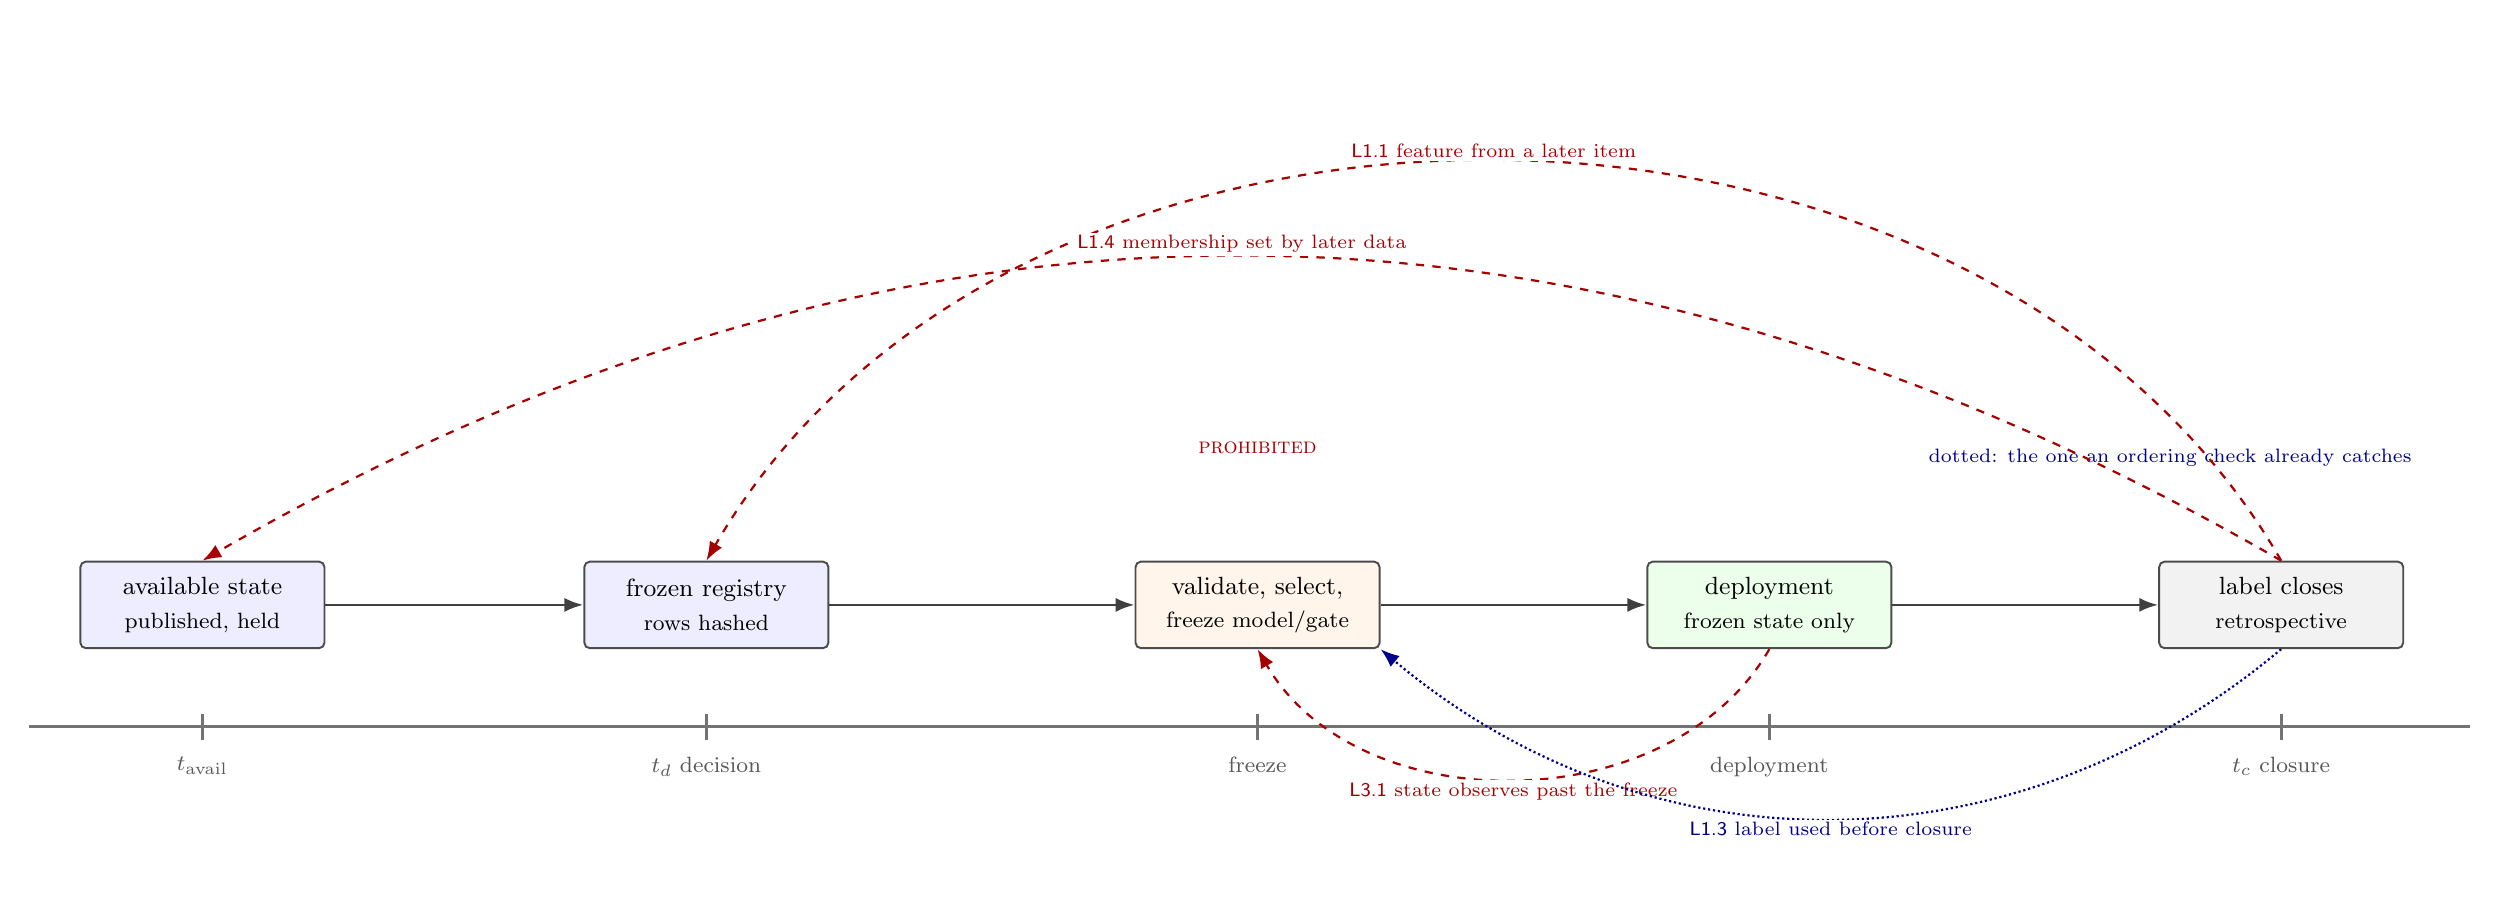
\begin{tikzpicture}[font=\small,>={Latex[length=2.4mm]},
  box/.style={draw=black!70,line width=0.7pt,rounded corners=2pt,align=center,
              minimum height=11mm,minimum width=31mm,inner sep=3pt,fill=white},
  ok/.style={->,line width=1.0pt,black!75},
  no/.style={->,line width=0.8pt,red!65!black,dashed},
  noord/.style={->,line width=0.8pt,blue!55!black,densely dotted}]
\draw[line width=1.1pt,black!55] (-0.6,0) -- (30.4,0);
\foreach \x/\lab in {1.6/{$t_{\text{avail}}$}, 8.0/{$t_d$ decision},
                     15.0/{freeze}, 21.5/{deployment}, 28.0/{$t_c$ closure}}
  {\draw[line width=1.1pt,black!55] (\x,-0.16) -- (\x,0.16);
   \node[font=\footnotesize,text=black!65,anchor=north] at (\x,-0.26) {\lab};}
\node[box,fill=blue!7]  (avail) at (1.6,1.55) {available state\\[1pt]\footnotesize published, held};
\node[box,fill=blue!7]  (reg)   at (8.0,1.55) {frozen registry\\[1pt]\footnotesize rows hashed};
\node[box,fill=orange!8](val)   at (15.0,1.55){validate, select,\\[1pt]\footnotesize freeze model/gate};
\node[box,fill=green!8] (dep)   at (21.5,1.55){deployment\\[1pt]\footnotesize frozen state only};
\node[box,fill=black!5] (lab)   at (28.0,1.55){label closes\\[1pt]\footnotesize retrospective};
\draw[ok] (avail) -- (reg); \draw[ok] (reg) -- (val);
\draw[ok] (val) -- (dep);   \draw[ok] (dep) -- (lab);
\node[font=\footnotesize,text=red!65!black,anchor=south] at (15.0,3.35)
  {\textsc{prohibited}};
\node[font=\scriptsize,text=blue!55!black,anchor=west] at (23.4,3.42)
  {dotted: the one an ordering check already catches};
\draw[no] (lab.north) to[out=120,in=60] node[pos=0.5,above,font=\scriptsize,
  fill=white,inner sep=1pt]{\rulename{L1.1} feature from a later item} (reg.north);
\draw[no] (lab.north) to[out=150,in=30] node[pos=0.5,above,font=\scriptsize,
  fill=white,inner sep=1pt]{\rulename{L1.4} membership set by later data} (avail.north);
\draw[no] (dep.south) to[out=-120,in=-60] node[pos=0.5,below,font=\scriptsize,
  fill=white,inner sep=1pt]{\rulename{L3.1} state observes past the freeze} (val.south);
\draw[noord] (lab.south) to[out=-140,in=-40] node[pos=0.5,below,font=\scriptsize,
  fill=white,inner sep=1pt]{\rulename{L1.3} label used before closure} (val.south east);
\end{tikzpicture}}
\caption{The deployment-causality contract. Solid paths are permitted: state available
before the decision instant $t_d$ populates a registry whose rows are frozen and
hashed, a model and admission decision are fixed at the freeze, deployment reads only
frozen state, and retrospective labels close afterwards. Prohibited paths are enforced by
named rules. The three \emph{dashed} paths are the point of this paper: each is
\emph{chronologically consistent} in the sense a train/validation/test split checks---the
timestamps are correctly ordered---so a split does not exclude them. The single
\emph{dotted} path (\rulename{L1.3}) is drawn for contrast: it \emph{is} an ordering
violation, and it is the one class a chronological split already catches.}
\label{fig:contract}
\end{figure*}


% Table I -- contract rules
% Included by paper/icc_main.tex via \input.
\begin{table*}[!t]
\caption{Contract rules. Every violation raises an exception carrying its rule
identifier. Detectors are two-sided: each has a clean-path test that passes and a
deliberately broken fixture that fails.}
\label{tab:rules}
\centering
\footnotesize
\begin{tabular}{@{}llp{4.6cm}p{4.3cm}l@{}}
\toprule
\textbf{Rule} & \textbf{Protected object} & \textbf{Violation example} &
\textbf{Mechanical check} & \textbf{Failure action}\\
\midrule
\rulename{L1.1} & feature availability & feature spans two past timestamps, one published later & recompute features with state after $t$ truncated; require bit-identity & halt \\
\rulename{L1.2} & availability clock & selection by descriptive rather than publication time & assert selected item's publication $\le t_d$ & halt \\
\rulename{L1.3} & label closure & label used before its closure time & mask by $t_c \le t_d$ & halt \\
\rulename{L1.4} & row membership & schedule extent taken from available data & rebuild from truncated source, same declared window & halt \\
\rulename{L1.5} & comparison boundary & availability test strict where it must be inclusive & probe before, exactly at, and after $t_d$ & halt \\
\rulename{L2.1} & sampling geometry & schedule sampled on a clock grid & assert every sample above the declared mask & halt \\
\rulename{L2.2} & physical scale & target below instrument resolution or above plausibility & ratio against a floor \emph{and} a ceiling & label, retain \\
\rulename{L2.3} & hidden state & error integrates over the window & late/early magnitude ratio & halt \\
\rulename{L2.4} & declared relation & config and code agree only where fitted & compare over domain \emph{plus} extrapolation margin & halt \\
\rulename{L3.1} & state channels & tracker observes outcomes past the freeze & six-channel mutation canary & halt \\
\rulename{L3.2} & canary effectiveness & probe mutation is a no-op & require the mutation to change an observable & halt \\
\rulename{L3.3} & negative control & zero-effect cell admits a learned branch & admission rate at every covariate level & halt \\
\rulename{L4.1} & fold chronology & folds overlap in time & compare fold time extents & halt \\
\rulename{L4.2} & paired randomness & condition label enters the seed & assert arms bit-identical off-intervention & halt \\
\rulename{L4.3} & repeated measures & replicates counted as observations & within-group correlation before aggregation & halt \\
\rulename{L4.4} & seed hygiene & burned seed re-enters evaluation & namespace disjointness & halt \\
\rulename{L4.5} & provenance hashes & artifact unhashed & manifest and self-hash present & halt \\
\rulename{L4.6} & provenance completeness & behaviour-changing input uncovered & differing outputs under one manifest hash & halt \\
\rulename{L4.7} & statistical unit & unit finer than the exchangeable one & residual correlation at the next coarser grouping & halt \\
\bottomrule
\end{tabular}
\end{table*}



\section{Orbit-Evidence Toolkit}

\emph{Engineering.} Three components support the rules and carry no argument of their own. The
\emph{visible-pass scheduler} emits transmissions only from intervals predicted by held state,
refining both elevation crossings to the above-mask side on the geodetic normal; the visibility
criterion and the solver settings both enter the provenance manifest. The
\emph{freeze-then-label registry} hashes rows against an absolute declared window before any label
source is consulted, and its falsifiable form compares registries built from full and truncated
data. The \emph{reference ensemble} publishes a median-absolute-deviation uncertainty and a closure
time with a coverage-only status---member count and spread against a declared ceiling, never the
labelled value---and never creates or deletes a row.

\subsection{Two rules that inspect a relation between runs}

\emph{Provenance completeness} (\rulename{L4.6}) cannot be verified by examining a manifest,
which is silent about what it omits---but it is verifiable differentially. Over input variations
$\{c_i\}$ producing output digests $o_i$ and manifest hashes $h_i$, any pair with
$o_i \neq o_j$ and $h_i = h_j$ proves the manifest incomplete, since two runs differing in
output must differ in provenance. The converse is not an error: identical outputs under
differing manifests is merely redundant. That asymmetry makes the rule checkable without
enumerating every input.

\emph{Statistical unit selection} (\rulename{L4.7}) asks not whether replicates were aggregated
but whether the level they were aggregated \emph{to} is exchangeable. Given values $y$, unit
identifiers $u$ and the next coarser grouping $g$ (for a satellite experiment: samples aggregated
to a pass, grouped by deployment episode), we aggregate to $\bar{y}_u$ and measure its intraclass
correlation \emph{within} $g$. Residual correlation there means the chosen unit shares state with
its neighbours, so intervals over it are optimistic.

The estimator is the unbiased one-way $\mathrm{ICC}(1)$ from variance
components~\cite{shrout1979icc}, expectation $0$ under independence at every group size. The
decision is referenced to a \emph{permutation null}: unit values are permuted across coarser
groups---the exchangeability hypothesis under test---giving
$p=(1+\#\{\hat{\rho}^{*}\ge\hat{\rho}\})/(B+1)$ over $B=\num{400}$ permutations at the observed
group count, halting at $p\le\alpha=0.05$. The $+1$ is not cosmetic: the $1-\alpha$ empirical
quantile is anticonservative by $1/(B+1)$, this form exact for any $B$. The reference distribution,
not the estimator, is what makes the decision calibrated---under the permutation null a raw
scatter ratio is a monotone transform of $\hat{\rho}$ and yields the same $p$. The estimator
matters for the reported value and for \rulename{L4.3}, which has no reference at all: at a fixed $0.2$ its measured null size is $0.17$ at eight groups of three, so it halts on about
one correct design in six. Because specificity is
a rate we measure it as one: over \artv{l47_clean_paths}{\num{450}} clean evaluations of this
rule alone (\num{150} seeds $\times$ three environments) it halts \artv{l47_false_halts}{\num{14}}
times, a rate of $\artv{l47_rate}{0.031}$ with Wilson~\cite{wilson1927} interval
$\artv{l47_wilson}{[0.018,0.052]}$---consistent with the nominal
$\artv{l47_alpha}{0.05}$, not better
than it---and it detects the injected fault on \num{150} of \num{150} paths. Two cautions. All \num{450} replicates sit at
eight groups of three balanced units, and the clean fixture satisfies the permutation null by
construction, so this measures the \emph{implementation}, not a rate that could have come out
otherwise. And rederiving the permutation stream moved the count \num{19}$\rightarrow$\num{14}
without touching the protocol: the interval is the claim, not the point. Finally the rule \emph{declines to judge} below four coarser groups holding two or more units
each, or eight units, returning \textsc{indeterminate} and raising nothing. That floor is a
\emph{power} precondition asserted on the design, not a validity one---the permutation test stays
size-valid at two groups; it simply cannot see anything there. That makes
the contract three-valued rather than two: \textsc{pass}, the condition is supported;
\textsc{halt}, it is violated; \textsc{indeterminate}, the design lacks the structure to decide.
Collapsing the third into the first is how an underpowered check comes to look like a satisfied
one. No condition in this suite is small enough to exercise it.

\emph{Canaries and seeds.} Six state channels are probed, separating whether a channel is
\emph{guarded} from whether the probe was \emph{effective}---an inert mutation reads as an
undetectable leak, which \rulename{L3.2} catches. Seeds live in three disjoint namespaces and one
whose outcomes have been inspected is burned for good; compared conditions draw one seed per
invariant cell, with pairing asserted on the realised arrays.

\section{Curated Regression Evaluation}
\label{sec:eval}

\subsection{Design}

Two pipelines serve as minimal deterministic fixtures. \textsc{Case A} exercises a
retrospective-label chain: held state, visible-pass scheduling, frozen registry, later reference
construction, closure. \textsc{Case B} exercises a learning and gating chain: physics baseline,
optional learned branch, validation selection, frozen model/scaler/gate state, later deployment.
Neither carries a physical claim.

The suite contains \num{17} \emph{curated} fault classes, drawn from the defects that motivated
the rules. Each is injected in three environments differing in pseudo-random generator family,
giving \num{51} injected cells, plus one clean reference path per environment reported separately.
Three denominators are easily conflated, so we fix them: \artv{rule_count}{\num{19}} \emph{rules}, \artv{fault_class_count}{\num{17}} fault
\emph{classes}, \num{18} \emph{conditions} per environment. Rules and classes are not in
bijection---one rule can be violated several ways, and some are represented by no fault here.

\subsection{Results}

Every number comes from one artifact,
\texttt{final\_summary.json}: Fig.~\ref{fig:opcurve} carries the measured operating
characteristic, Table~\ref{tab:rules} the coverage, Fig.~\ref{fig:cases} the counterexamples.
The chronological baseline is \emph{implemented and executed}, not reasoned about: three checks
assert that fold extents are ordered and disjoint, that no row sits in a fold whose span excludes
it, and that no label used at a decision postdates it, run in the same sweep over the same
fixtures. It is not a competing tool---chronological splitting is a \emph{protocol property}, so
this measures how much of the fault space that property covers.
Measured, it detects $\artv{chronological}{2/17}$ classes---invalid label-closure timing and a violated fold order,
precisely the two that \emph{are} ordering properties---and fires on no clean path; the remaining
fifteen lie outside what ordering can express. The contract detects $\artv{contract}{17/17}$, identically in all
three environments. We report \num{17} computations, not $51$, as the coverage denominator: the object handed to the
detector is bit-identical across environments for fourteen classes, so $\artv{injected_cells}{51/51}$ is a
\emph{determinism} statement, not seventeen results times three.

% Fig. 2 -- L4.7 operating characteristic.
% Included by paper/icc_main.tex via \input.
%
% This REPLACES the 17-class coverage matrix, which gave the largest visual allocation to
% the weakest result -- a matrix of assertions firing on inputs shaped to trip them.
%
% AXIS NOTE. An earlier version plotted the data at x = 5*ICC (the effect SD) while ticking the
% axis in ICC at x = 0,1,2,3 -- so the ticks labelled 0.5 and 0.8 sat at ICC 0.4 and 0.6, the
% curve ran past the end of its own axis, and reading power off the tick labelled 0.8 gave 0.87
% against a caption claiming 1.00. The x coordinate is now ICC itself. Keep it that way: if a
% point is added, give it an ICC coordinate, never an effect size.
%
% Every number below is read from evaluation/results/l47_power_curve.json and the
% l47_calibration block of final_summary.json, both regenerated by `make matrix`.
\begin{figure}[!t]
\centering
\resizebox{\columnwidth}{!}{%
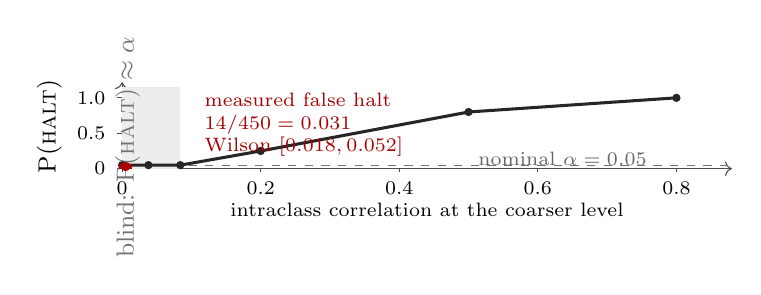
\begin{tikzpicture}[font=\footnotesize,x=88mm,y=9mm]
% axes. x runs past the last datum (ICC 0.8) so the curve ends inside its own axis.
\draw[->,black!70] (0,0) -- (0.88,0);
\draw[->,black!70] (0,0) -- (0,1.22);
\foreach \x/\lab in {0/{0}, 0.2/{0.2}, 0.4/{0.4}, 0.6/{0.6}, 0.8/{0.8}}
  {\draw[black!70] (\x,0) -- (\x,-0.04); \node[below,font=\scriptsize] at (\x,-0.05) {\lab};}
\foreach \y/\lab in {0/{0}, 0.5/{0.5}, 1/{1.0}}
  {\draw[black!70] (0,\y) -- (-0.008,\y); \node[left,font=\scriptsize] at (-0.010,\y) {\lab};}
\node[below,font=\scriptsize,align=center] at (0.44,-0.34)
  {intraclass correlation at the coarser level};
\node[rotate=90,font=\small] at (-0.105,0.6) {P(\textsc{halt})};
% low-correlation region: power is indistinguishable from size
\fill[black!7] (0,0) rectangle (0.084,1.15);
\node[font=\small,text=black!55,rotate=90,anchor=south] at (0.040,0.30)
  {blind: P(\textsc{halt}) $\approx\alpha$};
% nominal alpha reference
\draw[dashed,black!55] (0,0.05) -- (0.88,0.05);
\node[font=\scriptsize,text=black!60,anchor=west] at (0.50,0.135)
  {nominal $\alpha=0.05$};
% measured curve. x is ICC, y is measured P(HALT) over 40 seeds per point.
\draw[line width=1.1pt,black!85]
  (0.000,0.05) -- (0.010,0.05) -- (0.038,0.05) -- (0.084,0.05)
  -- (0.200,0.25) -- (0.500,0.80) -- (0.800,1.00);
\foreach \x/\y in {0.000/0.05, 0.038/0.05, 0.084/0.05, 0.200/0.25, 0.500/0.80, 0.800/1.00}
  {\fill[black!85] (\x,\y) circle (1.5pt);}
% the clean-path measurement, with its Wilson interval
\draw[line width=1.0pt,red!65!black] (0.005,0.018) -- (0.005,0.052);
\draw[line width=1.0pt,red!65!black] (-0.005,0.018) -- (0.015,0.018);
\draw[line width=1.0pt,red!65!black] (-0.005,0.052) -- (0.015,0.052);
\fill[red!65!black] (0.005,0.031) circle (1.7pt);
\node[font=\scriptsize,text=red!65!black,anchor=west,align=left] at (0.105,0.62)
  {measured false halt\\$14/450=0.031$\\Wilson $[0.018,0.052]$};
\end{tikzpicture}}
\caption{\rulename{L4.7}'s operating characteristic on one synthetic design (eight coarser groups
of three units). Specificity: \num{14} false halts over \num{450} clean replicates, $0.031$ against
nominal $0.05$ (red, Wilson interval)---consistent with $\alpha$, not better. Power: $1.00$ at
intraclass correlation $0.8$, $0.25$ at $0.2$, each over \num{40} seeds, decaying to the false-halt
rate below about $0.1$ (shaded). A gate needs both halves; specificity alone would hide that the
rule finds gross unit errors and misses subtle ones. Below four coarser groups or eight units it
returns \textsc{indeterminate}, not \textsc{pass}.}
\label{fig:opcurve}
\end{figure}


Clean reference paths were accepted: no rule fired on any of the three at the committed seed, and
clean verdicts were identical across environments. For the one rule with a stochastic reference
distribution the single clean run is not the evidence---the measured $0.031$ false-halt rate is.
\artv{red_fixture}{Sixteen} of nineteen rules are demonstrated red by a fault fixture; three (\rulename{L2.2},
\rulename{L2.3}, \rulename{L4.5}) are exercised only on the clean path. The full sweep runs in
under \qty{2}{\second} on one laptop core, under \qty{30}{\milli\second} per condition,
dominated by \rulename{L4.7}'s permutations. With \texttt{numpy} as the only dependency it is
affordable per commit rather than as a periodic audit.

One clean-path false positive was not designed: the first run reported three, all
\rulename{L4.4}, one per environment---caused by the fixture, not the detector, since the
clean pipeline declared it was about to execute a seed still in its own evaluation namespace.
We repaired the fixture, changed no detector, and preserved both records. The sequence
matters: adjusting the rule instead would have bought the clean-path rate by weakening the
contract.

\section{Two Chronology-Compliant Counterexamples}
\label{sec:cases}

Both pipelines come from a \emph{stopped} programme, were built with chronological splitting and
passed it. They motivate the model rather than evidence it: retrospective accounts predating the
contract, so we report which rule \emph{names} each defect rather than a halt we ran; no artifact
survives for the second; and the fixtures of \S\ref{sec:eval} were modelled on them, so
Table~\ref{tab:rules} and this section are not independent. No performance quantity is reported.

In the \emph{retrospective-label} pipeline, ordering guarantees every label postdates the
prediction it scores, and leaves three things unconstrained. A feature formed from the held and
\emph{reference} element epochs is a difference of two past timestamps---ordering-consistent, yet
built from an item the endpoint was never sent (\rulename{L1.1}). Row membership is conditioned on
the future catalogue, a transmission entering the dataset only if a qualifying later element was
published (\rulename{L1.4}). And label availability is coupled to the covariate under study,
because a publication outage simultaneously makes the held element stale and removes the elements
needed to label that staleness---so the comparison is undetermined, the baseline less tightly
pinned than the effect.

In the \emph{learning and gating} pipeline the feature tensor was clean and verified so by
perturbation, and ordering guarantees every training row predates every deployment row. What
crossed the freeze was not rows: a stateful tracker kept advancing at refresh events inside the
deployment window, so the learner observed outcomes after its own freeze (\rulename{L3.1}); the
negative control exposed undeclared deterministic signal, a rate frozen at one epoch against an
evolving reference (\rulename{L3.3}); and compared conditions failed to share a realisation, the
condition label having entered the seed derivation (\rulename{L4.2}). The tracker's update was
forward at every step and still wrong, which is what a row-level split cannot see.

% Fig. 3 -- case-study timelines
% Included by paper/icc_main.tex via \input.
% Node sublabels name the satellite-specific object each stage owns.
\begin{figure}[!t]
\centering
\resizebox{0.94\columnwidth}{!}{%
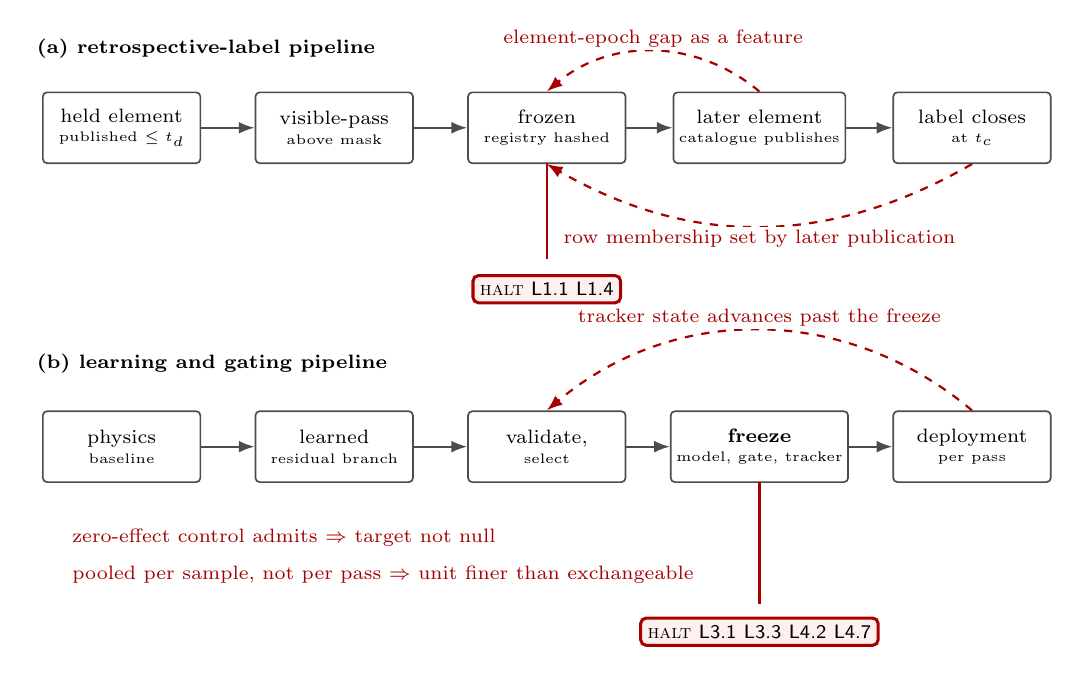
\begin{tikzpicture}[font=\scriptsize,>={Latex[length=2.0mm]},
  nd/.style={draw=black!70,line width=0.6pt,rounded corners=1.5pt,align=center,
             minimum height=9mm,minimum width=20mm,inner sep=2pt,fill=white},
  fl/.style={->,line width=0.8pt,black!70},
  bad/.style={->,line width=0.8pt,red!65!black,dashed},
  stop/.style={draw=red!65!black,line width=1.1pt,rounded corners=2pt,fill=red!6,
               align=center,inner sep=2.5pt,font=\scriptsize}]
% ---------------- panel (a)
\node[anchor=west,font=\scriptsize\bfseries] at (-0.3,2.05) {(a) retrospective-label pipeline};
\node[nd] (a1) at (0.9,1.05) {held element\\[-1pt]{\tiny published $\le t_d$}};
\node[nd] (a2) at (3.6,1.05) {visible-pass\\[-1pt]{\tiny above mask}};
\node[nd] (a3) at (6.3,1.05) {frozen\\[-1pt]{\tiny registry hashed}};
\node[nd] (a4) at (9.0,1.05) {later element\\[-1pt]{\tiny catalogue publishes}};
\node[nd] (a5) at (11.7,1.05) {label closes\\[-1pt]{\tiny at $t_c$}};
\foreach \x/\y in {a1/a2,a2/a3,a3/a4,a4/a5} \draw[fl] (\x) -- (\y);
\draw[bad] (a4.north) to[out=140,in=40]
  node[pos=0.5,above,font=\scriptsize,fill=white,inner sep=1pt]
  {element-epoch gap as a feature} (a3.north);
\draw[bad] (a5.south) to[out=-150,in=-30]
  node[pos=0.5,below,font=\scriptsize,fill=white,inner sep=1pt]
  {row membership set by later publication} (a3.south);
\node[stop] at (6.3,-1.0) {\textsc{halt} \rulename{L1.1} \rulename{L1.4}};
\draw[red!65!black,line width=0.9pt] (6.3,0.6) -- (6.3,-0.62);
% ---------------- panel (b)
\node[anchor=west,font=\scriptsize\bfseries] at (-0.3,-1.95) {(b) learning and gating pipeline};
\node[nd] (b1) at (0.9,-3.0) {physics\\[-1pt]{\tiny baseline}};
\node[nd] (b2) at (3.6,-3.0) {learned\\[-1pt]{\tiny residual branch}};
\node[nd] (b3) at (6.3,-3.0) {validate,\\[-1pt]{\tiny select}};
\node[nd] (b4) at (9.0,-3.0) {\textbf{freeze}\\[-1pt]{\tiny model, gate, tracker}};
\node[nd] (b5) at (11.7,-3.0) {deployment\\[-1pt]{\tiny per pass}};
\foreach \x/\y in {b1/b2,b2/b3,b3/b4,b4/b5} \draw[fl] (\x) -- (\y);
\draw[bad] (b5.north) to[out=140,in=40]
  node[pos=0.5,above,font=\scriptsize,fill=white,inner sep=1pt]
  {tracker state advances past the freeze} (b3.north);
\node[font=\scriptsize,text=red!65!black,anchor=west] at (0.15,-4.15)
  {zero-effect control admits $\Rightarrow$ target not null};
\node[font=\scriptsize,text=red!65!black,anchor=west] at (0.15,-4.62)
  {pooled per sample, not per pass $\Rightarrow$ unit finer than exchangeable};
\node[stop] at (9.0,-5.35) {\textsc{halt} \rulename{L3.1} \rulename{L3.3}
  \rulename{L4.2} \rulename{L4.7}};
\draw[red!65!black,line width=0.9pt] (9.0,-3.45) -- (9.0,-5.0);
\end{tikzpicture}}
\caption{Where the contract halts each case study, with the satellite object each stage owns
named beneath it: element publication versus epoch, visible-pass scheduling, the frozen
registry fixing row membership, frozen model/gate/tracker state, and the pass as statistical
unit. Solid arrows are the intended flow, dashed the defects found. Every dashed path is
chronologically consistent, which is why ordering does not exclude it. No model-performance
quantity is reported from either pipeline.}
\label{fig:cases}
\end{figure}


\section{Threats to Validity, Limitations and Conclusion}
\label{sec:threats}

\emph{The faults and the rules share an origin}: both were developed in one programme, mostly by
the same hand, so $17/17$ measures detector \emph{reachability}---a fixture written to trip rule
$X$ trips rule $X$---not mutation adequacy~\cite{jia2011mutation}, and hand-authored mutants are
known to overstate suite strength~\cite{just2014mutants}. Only one fault was specified before any detector for it existed, far too few to support a claim about faults the suite lacks, so we make none. What it establishes is regression coverage of \emph{represented} faults: these violations, once fixed, cannot silently return. The denominator is curated, not sampled.

\emph{Injection is at contract-input level.} The fixtures hand every rule its own input attribute:
of the seventeen mutated objects only six reach more than one consumer---and in all six that
consumer is another check, never a computation producing a reported number---so for the other eleven a
condition shows a rule firing on a broken input rather than catching a defect in a working
pipeline. This is the sharpest limit on the evaluation. \rulename{L2.2}, \rulename{L2.3} and
\rulename{L4.5} fire in no condition at all, which by our own standard is not evidence they
\emph{can} fail.

\emph{Four rules are weaker than their statement.} \rulename{L4.6} draws its power from the
caller's variation set, so it refutes a manifest omitting an input already suspected; the input
nobody thought of is absent from the sweep by construction, and the non-circular form perturbs the
environment blanketly, as build tooling does. \rulename{L4.3} is gated on a self-reported flag, so
a pipeline declaring itself aggregated silences it, and it still uses the fixed threshold whose
null size we measured at $0.17$. \rulename{L4.5} checks that a manifest and self-hash exist, not
that either is correct. And \rulename{L4.7}, though size-controlled, has power only against gross
unit errors.

\emph{Three objects the contract names but does not check.} Covariate-coupled label availability,
called the harder failure in \S\ref{sec:whysat}, has no rule and no fault: it was found by an
\emph{ad hoc} thresholded diagnostic---a standardised mean difference between labelled and censored
rows on pre-decision covariates, which fired in the stopped pipeline of \S\ref{sec:cases} and is
recorded in the archived audit---never promoted, so it has no identifier and no red fixture. $t_d$
is declared, not checked: under periodic provisioning the defensible $t_d$ is the refresh instant,
and declaring the transmission instant lets every availability check pass while admitting a refresh
interval of unheld state. And the availability clock is instrumented with an
optimistic proxy: \texttt{CREATION\_DATE} is when a message was \emph{created}, a lower bound on
when it could be \emph{retrieved}---batch publication and reprocessing add unmeasured lag---so
\rulename{L1} has one-sided error, able to pass a feature that was in fact unavailable but never
to fail one that was available. Epoch~$\le$~publication is likewise unchecked and sometimes
false, and applying our own \rulename{L4.7} question to our own statistic changes it: pooled over
\artv{lag_records}{\num{63727}} records the epoch leads publication in
\qty{\artv{lag_pooled_epoch_ahead_pct}{27.6}}{\percent} of cases, but one object supplies
\qty{\artv{lag_largest_object_share_pct}{82}}{\percent} of them and is the only object where it
happens at all---per object the figure is $0$ in ten of eleven. The record is the wrong unit here,
as it is in the experiments the contract governs. At the object level the premise is \emph{stronger}
than the pooled view suggested: the median publication lag is
\qty{\artv{lag_object_median_h}{6.36}}{\hour} rather than
\qty{\artv{lag_pooled_median_h}{1.68}}{\hour}, and positive for all eleven.

\emph{The axes of variation are narrow.} Both fixtures come from this programme, so reuse across independent projects is argued rather than demonstrated, and environments differ in generator family alone. No radio-frequency, packet-level or learned-method result is established here. Nor is the contract complete: six protected objects and six state channels are operational
enumerations, not completeness claims. \rulename{L4.7} also presumes a \emph{unique} next coarser
level, and orbital data does not supply one---element sets and deployment episodes cross-cut rather
than nest, and the rule tests whichever grouping the caller declares, so a design exchangeable at
one may not be at the other. The level we omit is the one most likely to matter: drag mismodelling
driven by solar and geomagnetic activity is common-mode across every object and element set in an
interval, so an experiment exchangeable at the element set can still fail at the space-weather
level. A regression suite protects exactly what it represents: showing a rule catches defects nobody anticipated needs faults authored independently of the detectors and injected at program level.

The lesson is not that a longer checklist replaces a temporal split, but that some validity
obligations are \emph{relational}: they concern how two executions differ, or whether the chosen
unit stays exchangeable one physical level coarser. Making those executable---and letting the gate
abstain when the design cannot support a decision---turns an assumption into a claim CI can
enforce. Satellite software is where we found them because it separates the clocks, the geometry
and the publisher a single-table view hides. We have shown the checks fire on the violations we
represented, cheaply enough for every commit; what remains is to run them against faults, and
pipelines, we did not write.

\bibliographystyle{IEEEtran}
\bibliography{refs}

\end{document}
